%%%%%%%%%%%%%%%%%%%%%%%%%%%%%%%%%%%%%%%%%%%%
% 
% Last edits: Nov 9, 2016
%%%%%%%%%%%%%%%%%%%%%%%%%%%%%%%%%%%%%%%%%%%%

\documentclass[12pt]{article}
\usepackage{natbib}
\usepackage[letterpaper, margin=1in]{geometry}
\usepackage{graphicx}
\usepackage[table,xcdraw]{xcolor}
\usepackage{wrapfig}
\usepackage{enumitem}
\setlist[enumerate]{itemsep=0mm}
\usepackage{multirow}
\usepackage{lscape}
\usepackage{caption}
\usepackage{subcaption}
\usepackage{float}
\usepackage{hyperref}


\begin{document}
\noindent{Alexandra Pulwicki \\ \today}

\begin{center}
\Large \textbf{Results\\ Observations}
\end{center}


\section*{Overview}

This document shows an overview of the data that is available for the project. It provides a first look at the processed data and provides figures that visualize the data. Section 1 examines the density data and uncertainty and potential systematic errors associated with measurements made in the snowpits and using a Federal Sampler. Section 2 briefly looks at the snow depths measured at the study glaciers. Section 3 visualizes the collected zigzag data. Section 4 examines the various ways to estimate snow water equivalent (SWE) at each measurement location. It focuses on options for how to interpolate density measurements and then visualizes estimated SWE at the measurement locations. 


\tableofcontents
\pagebreak



%%%
\section{Density Estimates}
%%%

\subsection{Basic statistics}

A summary of density data collected in snowpits and when using a Federal Sampler can be seen in Table \ref{tab:density_stats}. The standard deviation of each type of density measurement is less than 10\% of the mean density. For snowpit derived densities, the mean density is indistinguishable between glaciers within one standard deviation. The densities estimated using the Federal Sampler differed with one standard deviation. Glacier 2 had a lower density than Glacier 4, while Glacier 13 had the same density as both. The mean of all Federal Sampler density values was likely skewed by the proportionally large number of measurements obtained on Glacier 13.

\begin{table}[h!]
\centering
\caption{ Mean and standard deviation (std) of snow density (kg m$^{-3}$) measured on study glaciers in snowpits and using a Federal Sampler. The number of sampling locations ($n$) is also given.}
\label{tab:density_stats}
\begin{tabular}{c|ccc|ccc}
 & \multicolumn{3}{c}{\textbf{Snowpits}} & \multicolumn{3}{|c}{\textbf{Federal Sampler}} \\
\multirow{-2}{*}{\textbf{Glacier}} & Mean & Std & n & Mean & Std & n \\ \hline \hline
\textbf{Glacier 4} & 348 & 13 & 3 & 355 & 18 & 7 \\
\textbf{Glacier 2} & 333 & 26 & 4 & 286 & 34 & 7 \\
\textbf{Glacier 13} & 349 & 26 & 3 & 316 & 40 & 17 \\  \hline
\textbf{All} & 342 & 26 & 10 & 318 & 42 & 31
\end{tabular}
\end{table}

\subsection{Federal Sampler measurements and snow depth}

\begin{wrapfigure}[18]{l}{0.6\textwidth} 
	\centering
	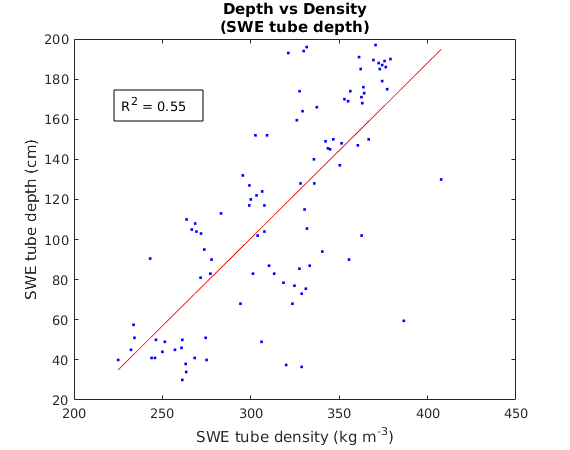
\includegraphics[width =0.6\textwidth]{DepthDensity_SWEtube.png}\\
	\caption{Linear regression of measured snow density and depth for all Federal Sampler measurements.}
	\label{fig:tube_depth}
\end{wrapfigure}

A plot of measured SWE and snow depth can be seen in Figure \ref{fig:tube_depth}. A positive linear relation exists (R$^2$ = 0.59, p$<$0.01). This positive relationship could be a result of physical processes, such as compaction, and/or artefacts during data collection however, it seems more likely that this trend is a result measurement artefacts for a number of reasons. First, the range of densities measured by the Federal sampler is large (225--410 kg m$^{-3}$) and the extreme values seem unlikely to exist at these study glaciers, which experience a continental snowpack with minimal mid-winter melt events. Second, compaction effects would likely be small at these study glaciers because of the relatively shallow snowpack (deepest measurement was 340 cm). Third, no linear relationship exists between depth and snowpit-derived density (R$^2$ = 0.05) as can be seen in a plot of the depth-density relationship in snowpits in Figure \ref{fig:pit_depth}. A plot of both Federal Sampler measurements and snowpit measurements can be seen in \ref{fig:all_depth}. Together, these reasons lead to the likely conclusion that the Federal Sampler measurements are biased. 
 
 \begin{wrapfigure}[17]{t}{0.55\textwidth} 
	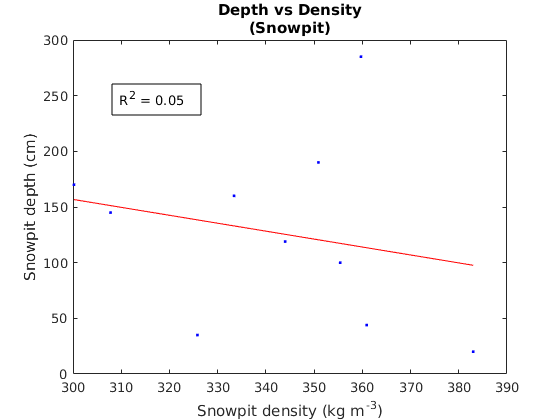
\includegraphics[width =0.55\textwidth]{DepthDensity_SP.png}\\
	\caption{Relationship between measured density and snow depth for all snowpit locations.}
	\label{fig:pit_depth}
\end{wrapfigure}

To account for this likely artefact, the simplest form of linear detrending can be applied. The linear fit was subtracted from each data point and the original data mean was added to each point. A plot of the detrended density data can be seen in Figure \ref{fig:tube_depthDETREND}. This detrended data will not be used for subsequent analysis but can be accessed by changing \texttt{options.TubeDensity} accordingly.

\begin{figure}[p]
	\centering
	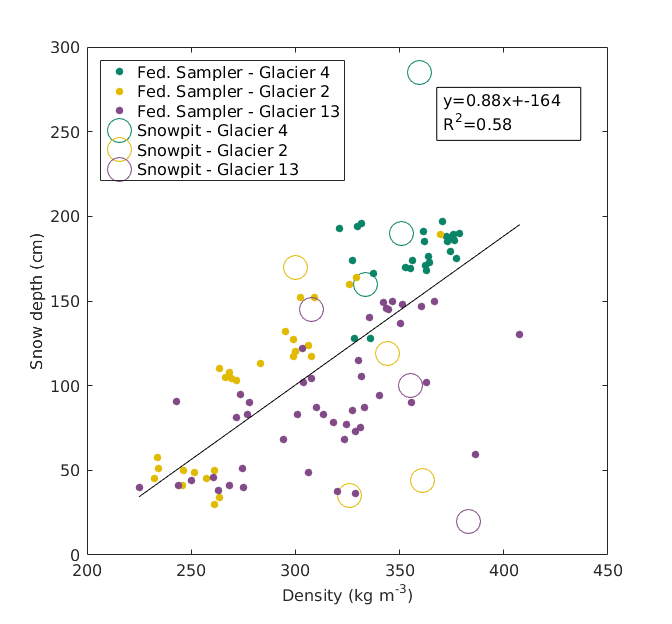
\includegraphics[width =0.7\textwidth]{DepthDensity_SWEonly.png}\\
	\caption{Relationship between measured density and snow depth for all Federal Sampler and snowpit locations.}
	\label{fig:all_depth}

	\centering
	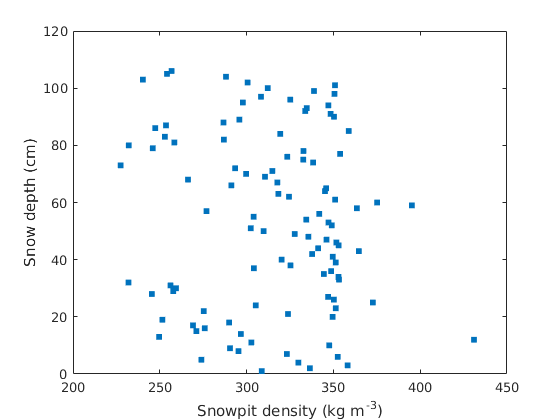
\includegraphics[width =0.7\textwidth]{DepthDensity_tubeDETREND.png}\\
	\caption{Plot of depth-detrended density and snow depth for all Federal Sampler measurements.}
	\label{fig:tube_depthDETREND}
\end{figure}



\subsection{Density uncertainties}

\subsubsection{Snowpit density}

Uncertainty in estimating density from snowpits is likely dominated by measurement errors and incorrect assumptions of density of layers that could not be sampled (i.e. ice lenses and `hard' layers). To determine a possible range of density values from snowpit measurements, the original data was used and three parameters were varied. Ice layer density was varied between 700 and 900 kg m$^{-3}$, ice layer thickness was varied by $\pm$1 cm, and the density of layers identified as being too hard to sample (but not ice) was varied between 600 and 700 kg m$^{-3}$. 

The resulting minimum and maximum possible densities for each snowpit can be seen in Table \ref{tab:density}. The range of density values is always less than 15\% of the reference density, with the largest ranges present on Glacier 2. Density values for shallow pits that contained ice lenses were particularly sensitive to changes in density and ice lens thickness. 

\begin{table}[]
\centering
\caption{Summary of assumed and range of integrated snow density calculated in snowpits. The assumed density values arose from taking a density of 917 kg m$^{-3}$ was applied to ice layers and a density of 600 kg m$^{-3}$ was applied to layers that were described as `hard' and were too difficult to sample. To determine the error in estimating integrated snow density, the values of ice density, ice thickness, and the `hard' layer density was varied between 700 and 917 kg m$^{-3}$, $\pm$ 1 cm, and 500 and 600 kg m$^{-3}$, respectively.}
\label{tab:density}
\resizebox{\textwidth}{!}{%
\begin{tabular}{lcccccc}
 &  & \multicolumn{4}{c}{\textbf{Density (kg m$^{-3}$)}} &  \\
\multirow{-2}{*}{} & \multirow{-2}{*}{\textbf{Depth (m)}} & \textit{Assumed value} & \textit{Minimum} & \textit{Maximum} & \textit{Range} & \multirow{-2}{*}{\textbf{\begin{tabular}[c]{@{}c@{}}Range as \% \\ of assumed value\end{tabular}}} \\ \hline \hline
G02\_LSP & 44 & 360.9 & 328.6 & 377.3 & 48.7 & 13.5 \\
G02\_Z4A\_SWE & 35 & 325.8 & 307.9 & 344.7 & 36.8 & 11.3 \\
G02\_USP & 119 & 344.0 & 327.1 & 361.9 & 34.8 & 10.1 \\ 
G02\_ASP & 170 & 300.2 & 298.6 & 303.1 & 4.5 & 1.5 \\  \hline
G04\_LSP & 190 & 350.9 & 343.2 & 359.1 & 15.9 & 4.5 \\
G04\_USP & 160 & 333.4 & 316.6 & 349.6 & 33.0 & 9.9 \\
G04\_ASP & 285 & 359.7 & 356.6 & 362.4 & 5.8 & 1.6 \\  \hline
G13\_LSP & 20 & 383.0 & 383.0 & 383.0 & 0 & 0 \\
G13\_USP & 100 & 355.4 & 345.6 & 366.9 & 21.3 & 6.0 \\
G13\_ASP & 145 & 307.8 & 306.4 & 308.2 & 1.8 & 0.6
\end{tabular}%
}
\end{table}

\subsubsection{Federal Sampler densities}

Density values estimated from Federal Sampler measurements are shown in Table \ref{tab:density_TubeRange}. Mean density has a larger spread of values over the study glaciers when compared to snowpit densities. The \% range is also larger than snowpit densities for many of the measurement locations. 

\begin{table}[]
\centering
\caption{Range of densities estimated from Federal Sampler measuresments. The number ($n$) of good quality measurements, as well as the minimum, maximum, and mean density are shown. The density range given as a percent of the mean density is also shown.}
\label{tab:density_TubeRange}
\begin{tabular}{lccccc}
\multicolumn{1}{c}{\multirow{2}{*}{\textbf{Location}}} & \multirow{2}{*}{\textbf{$n$}} & \multicolumn{3}{c}{\textbf{Density (kg m$^{-3}$)}} & \multirow{2}{*}{\textbf{\begin{tabular}[c]{@{}c@{}}Range as \%\\ of mean (\%)\end{tabular}}} \\
\multicolumn{1}{c}{} &  & Mean & Minimum & Maximum &  \\ \hline  \hline
G04\_Z3A\_SWE & 3 & 334 & 309 & 358 & 14 \\
G04\_USP & 6 & 311 & 274 & 353 & 22 \\
G04\_Z2A\_SWE & 3 & 360 & 303 & 431 & 35 \\
G04\_LSP & 7 & 272 & 250 & 297 & 13 \\
G04\_Z5B\_SWE & 2 & 337 & 324 & 350 & 7 \\
G04\_Z5A\_SWE & 3 & 311 & 275 & 351 & 21 \\
G04\_Z5C\_SWE & 2 & 361 & 350 & 373 & 6 \\  \hline
G02\_Z5C\_SWE & 2 & 296 & 245 & 347 & 28 \\
G02\_USP & 7 & 294 & 232 & 353 & 34 \\
G02\_Z7A\_SWE & 3 & 326 & 304 & 349 & 12 \\
G02\_Z7B\_SWE & 2 & 336 & 320 & 351 & 9 \\
G02\_Z7C\_SWE & 3 & 351 & 338 & 365 & 7 \\
G02\_Z3B\_SWE & 3 & 349 & 341 & 353 & 3 \\
G02\_LSP\_SWE & 7 & 331 & 302 & 349 & 13 \\ \hline
G13\_ASP & 8 & 343 & 277 & 395 & 33 \\
G13\_651 & 3 & 329 & 318 & 345 & 7 \\
G13\_652 & 2 & 319 & 291 & 346 & 15 \\
G13\_654 & 3 & 298 & 266 & 318 & 14 \\
G13\_655 & 1 & 300 & 300 & 300 & 0 \\
G13\_656 & 3 & 279 & 227 & 315 & 24 \\
G13\_657 & 3 & 331 & 323 & 338 & 4 \\
G13\_658 & 2 & 343 & 333 & 354 & 6 \\
G13\_659 & 3 & 245 & 232 & 258 & 7 \\
G13\_Z7C\_SWE & 2 & 270 & 253 & 287 & 9 \\
G13\_USP & 6 & 294 & 247 & 359 & 31 \\
G13\_Z4C\_SWE & 4 & 342 & 334 & 350 & 5 \\
G13\_744 & 3 & 323 & 298 & 347 & 14 \\
G13\_Z3B\_SWE & 3 & 333 & 308 & 351 & 12 \\
G13\_Z4B\_SWE & 2 & 332 & 312 & 351 & 11 \\
G13\_Z5A\_SWE & 3 & 276 & 240 & 301 & 17 \\
G13\_Z5B\_SWE & 2 & 255 & 254 & 257 & 1
\end{tabular}
\end{table}

\subsection{Comparing density from snowpit and Federal Sampler measurements}

To compare snowpit-derived densities and Federal Sampler-derived densities, eight Federal Sampler measurements were taken around two snowpit locations on each study glacier. The results are shown in Figure \ref{fig:density_pitVStube}. The overall range of Federal Sampler-derived densities is larger than that of the snowpit-derived density values. Within the range of possible values (minimum and maximum densities), the density values are indistinguishable for all snowpit locations, except for the accumulation snowpit on Galcier 13 (`G13\_ASP').

\begin{figure}[H]
	\centering
	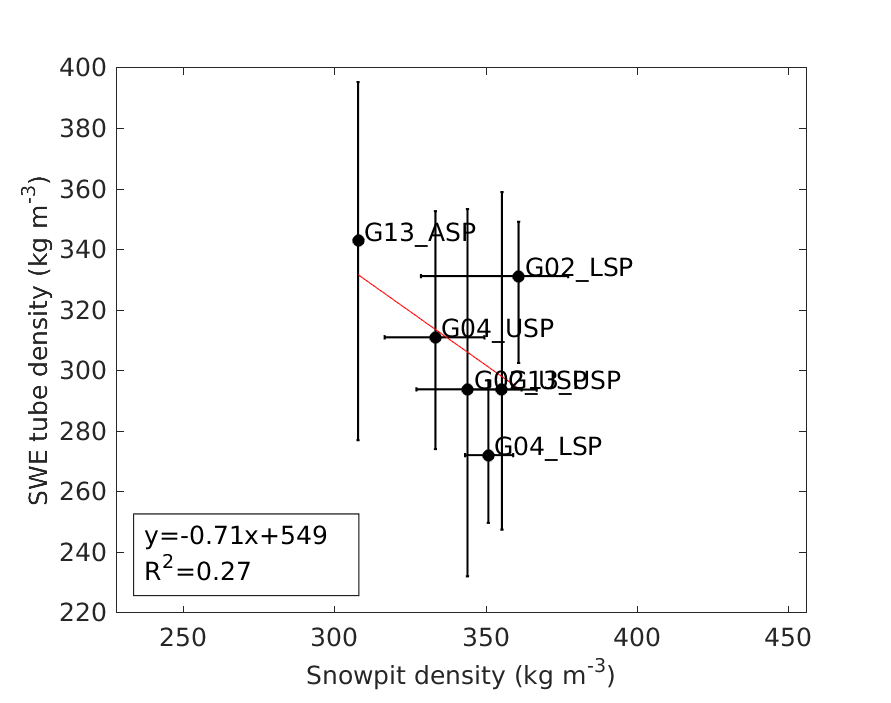
\includegraphics[width =0.95\textwidth]{SnowpitVsSWEtube_all.png}\\
	\caption{Comparison of density estimated using wedge cutters in a snow pit and Federal Sampler measurements for three study glaciers. Error bars are minimum and maximum values for each estimate as seen in Table \ref{tab:density} and \ref{tab:density_TubeRange}. A 1:1 reference line is also shown.}
	\label{fig:density_pitVStube}
\end{figure}


\subsection{Density and elevation}

A linear fit between density and elevation is often used to interpolate density values between measurement locations. A summary of linear fits of the snowpit-derived and Federal Sampler-derived densities can be seen in Table \ref{tab:elev_regress}. There seems to be no generalization of elevation regressions between study glaciers and even between sampling methods. Note that since Federal Sampler measurements, which have been shown to have a significant relationship between snow depth and estimated density, are likely to have skewed regressions because snow depth is significantly correlated with elevation (as seen in Figure \ref{fig:depth_elev}). 

A plot of snowpit-derived density versus elevation can be seen in Figure \ref{fig:elev_snowpit} and a plot of Federal Sampler-derived density versus elevation can be seen in Figure \ref{fig:elev_tube}.


\begin{table}[]
\centering
\caption{Summary of linear regressions between snowpit-derived density and elevation ($z$) as well as Federal Sampler-derived densities and elevation ($z$) for the study area.}
\label{tab:elev_regress}
\begin{tabular}{lcccc}
\multicolumn{1}{c}{} & \multicolumn{2}{c}{\textbf{\begin{tabular}[c]{@{}c@{}}Snowpit \\ Regression\end{tabular}}} & \multicolumn{2}{c}{\textbf{\begin{tabular}[c]{@{}c@{}}Fed. Sampler\\ Regression\end{tabular}}} \\
\multicolumn{1}{c}{\multirow{-2}{*}{\textbf{Location}}} & Equation & R$^2$ & Equation & R$^2$ \\ \hline  \hline
Glacier 4 & 0.03$z+$274 & 0.16 & -016$z+$714 & 0.53 \\
Glacier 2 & -0.14$z+$659 & 0.75 & 0.24$z-$282 & 0.72 \\
Glacier 13 & -0.19$z+$796 & 1.00 & 0.12$z+$33 & 0.21 \\ \hline
All & -0.12$z+$618 & 0.50 & -0.14$z+$659 & 0.75
\end{tabular}
\end{table}


\begin{figure}[H]
  \makebox[\textwidth][c]{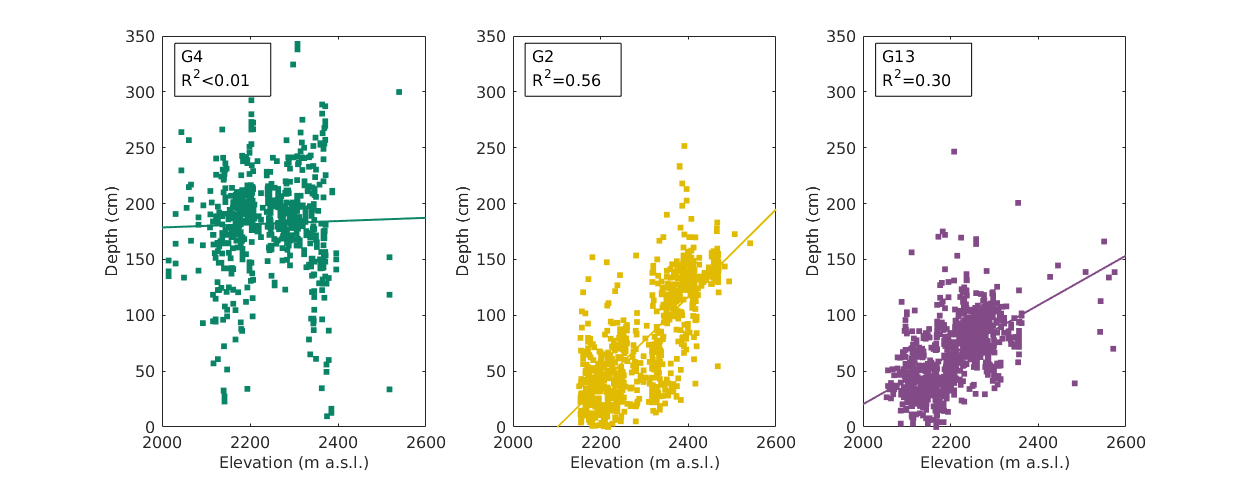
\includegraphics[width=1.2\textwidth]{DepthElevation.png}}%
	\caption{Relationship between measured snow depth and elevation at all sampling locations.}
	\label{fig:depth_elev}
\end{figure}


\begin{figure}[H]
	\centering
	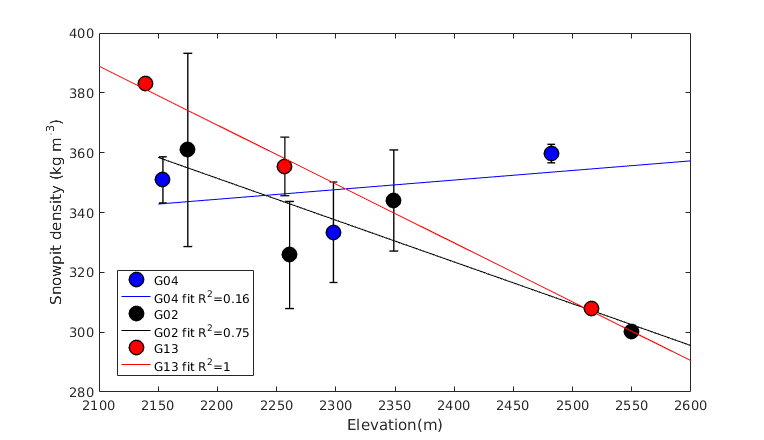
\includegraphics[width = 0.7\textwidth]{ElevationVsSnowpit_all.png}\\
	\caption{Relationship between snowpit-derived density and elevation for all study glaciers.}
	\label{fig:elev_snowpit}
\end{figure}


\begin{figure}[H]
	\centering
	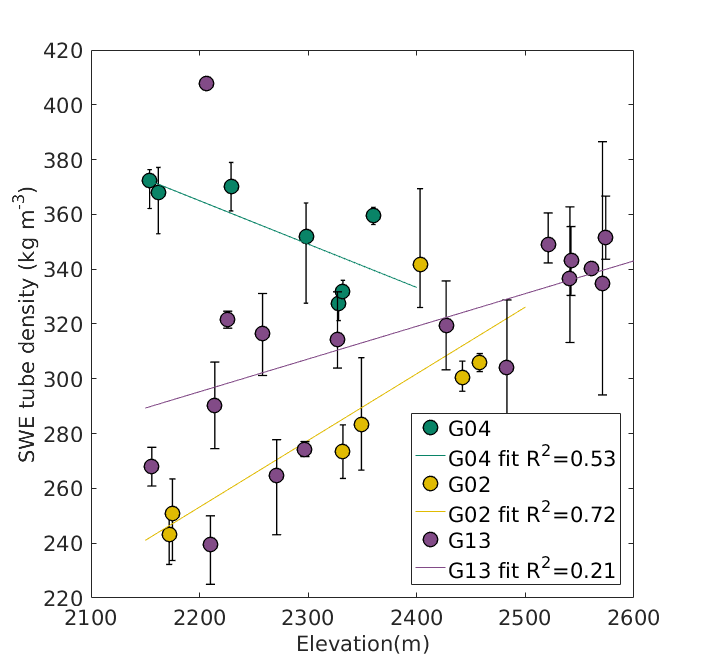
\includegraphics[width = 0.6\textwidth]{ElevationVsSWEtube_all.png}\\
	\caption{Relationship between Federal Sampler-derived density and elevation for all study glaciers.}
	\label{fig:elev_tube}
\end{figure}


\pagebreak

%%%%%%%%%%%%%%%%%%%%%%%%%%%%%%%%%%%%%%
\section{Snow depth}

\begin{figure}[H]
    \centering
    \begin{subfigure}[b]{0.48\textwidth}
        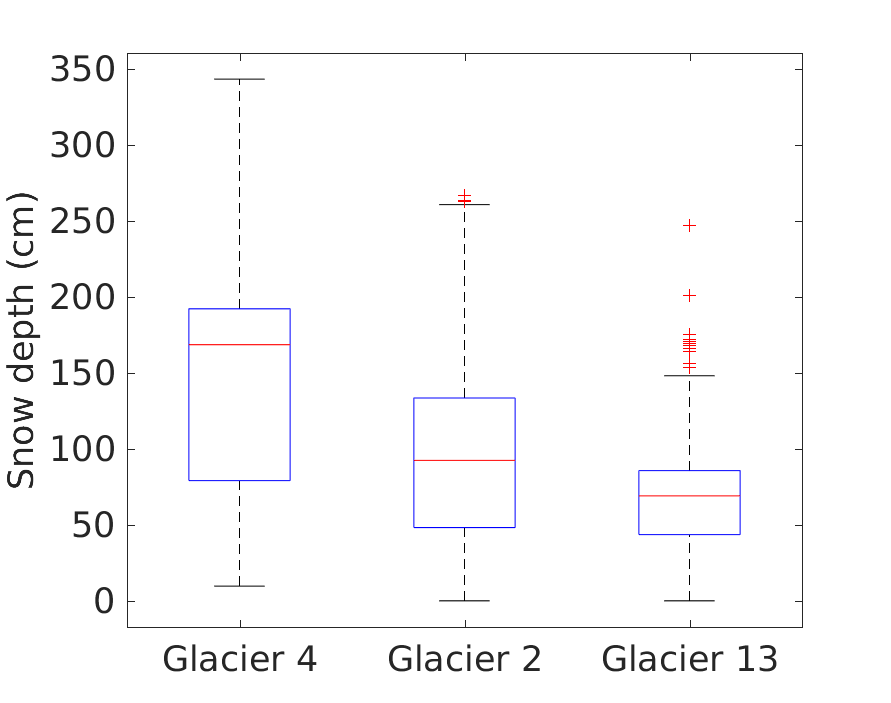
\includegraphics[width=\textwidth]{box_depth_wZZ.png}
        \caption{ }
        \label{fig:box_depth_wZZ}
    \end{subfigure}
    ~
    \begin{subfigure}[b]{0.48\textwidth}
        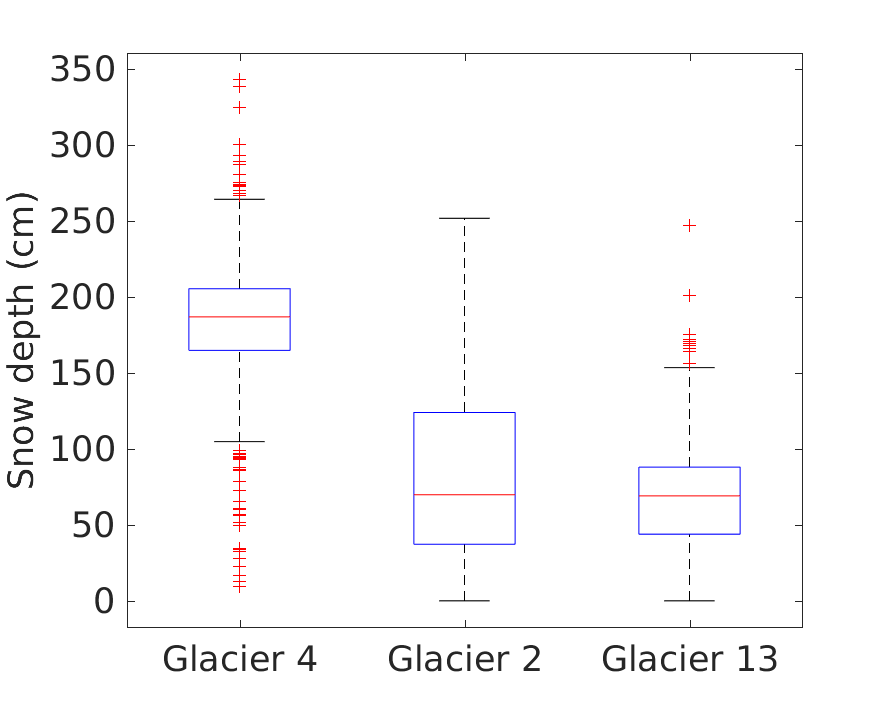
\includegraphics[width=\textwidth]{box_depth_noZZ.png}
        \caption{}
        \label{fig:box_depth_noZZ}
    \end{subfigure}

    \caption{Boxplots of snow depth measured on study glaciers. All snow depth values shown in (a) and snow depth values only from transects shown in (b). Red line indicates median, blue box shows first quantiles (25th and 75th percentiles), bars indicate minimum and maximum values (excluding outliers), and red crosses show outliers, which are defined as being outside of the range of 1.5 times the quartiles (approximately $\pm2.7\sigma$).}
    \label{fig:box_depth}
\end{figure}

A summary of the measured snow depth on all study glaciers is shown in Figure \ref{fig:box_depth} where \ref{fig:box_depth_wZZ} shows all snow depth measured (including zigzag values) and \ref{fig:box_depth_noZZ} shows snow depth values collected along curvilinear and linear transects. In both cases, Glacier 4 has the largest median and range of snow depth values, while Glacier 13 has the smallest. 

\pagebreak
%%%%%%%%%%%%%%%%%%%%%%%%%%%%%%%%%%%%%%
\section{Zigzag data}

A comparison of measured snow depth for each zigzag is shown in Figure \ref{fig:ZZ_boxplot}. The zigzags on Glacier 4 show minimal variability with a small range of values observed and few outliers. The mean depth is significantly larger at the upper most zigzag. Zigzags on Glacier 2 show more variability. The range on the mid zigzag is the largest of all the zigzags measured and the highest zigzag has many outliers. The zigzags on Glacier 13 do not vary considerably in range, although the lower zigzags show a large number of outliers which may be a results of these locations being close to a supraglacier meltwater channel. 

The depth measured at each zigzag is shown in Figures \ref{fig:ZZ_G04}, \ref{fig:ZZ_G02}, and \ref{fig:ZZ_G13}. There is considerable variability both between zigzags and within each zigzag. For example, in Figure \ref{fig:ZZ_G04}, `G04\_Z5B' has a more uniform snow depth than `G04\_Z3A', which has a large range in depth values. 
{
\begin{wrapfigure}{r}{1.1\textwidth} 
	\centering
	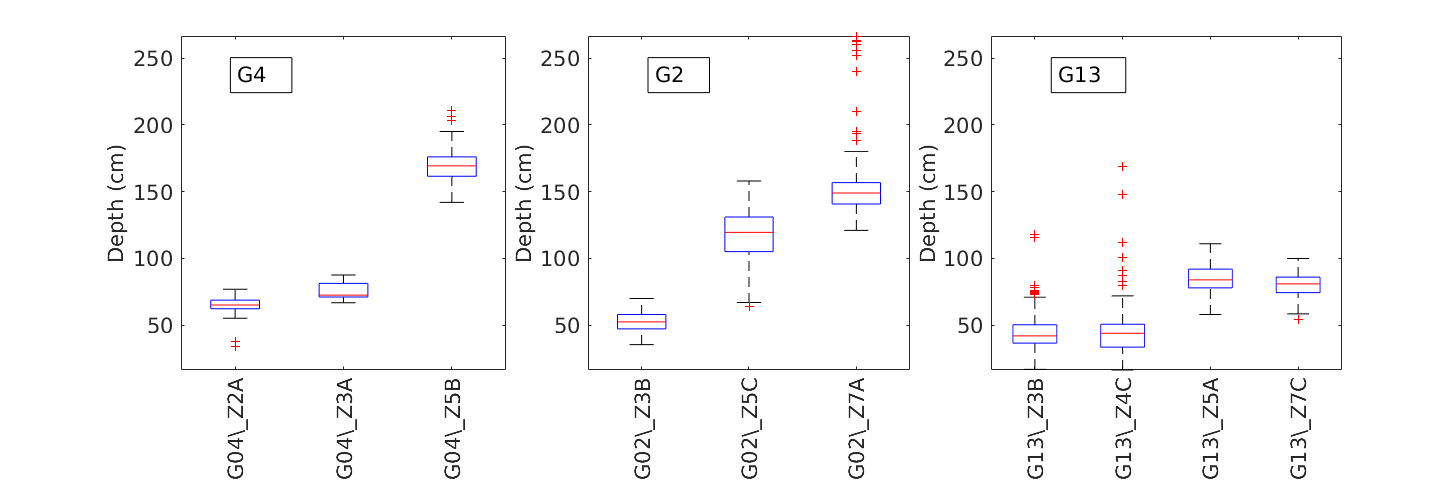
\includegraphics[width = 1.1\textwidth]{Zigzag_Boxplot.png}\\
	\caption{Boxplot of zigzag depths measured at each zigzag location.}
	\label{fig:ZZ_boxplot}
\end{wrapfigure}
}

\begin{landscape}
\begin{figure}
	\centering
	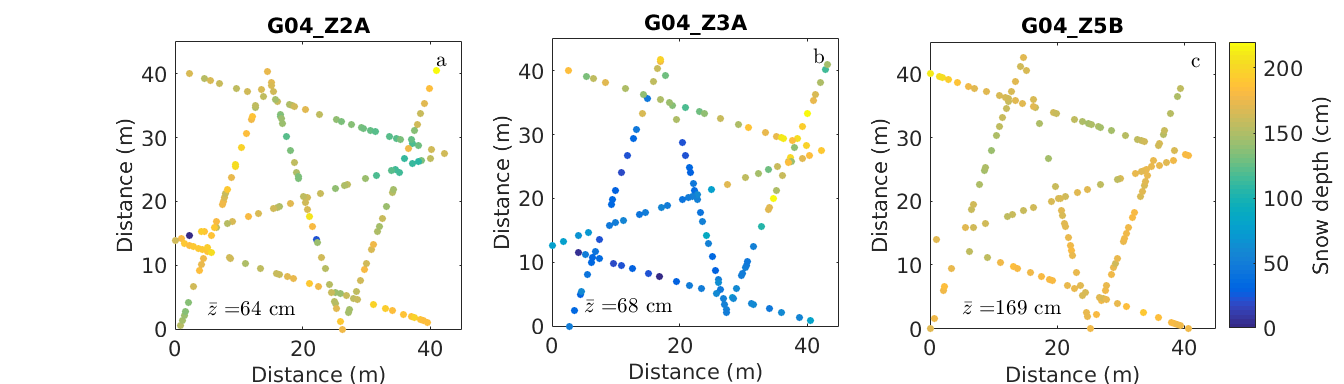
\includegraphics[width = 23 cm]{ZigzagDepth_G04.png}\\
	\caption{Plot of depth measured at zigzags on Glacier 4.}
	\label{fig:ZZ_G04}
\end{figure}

\begin{figure}
	\centering
	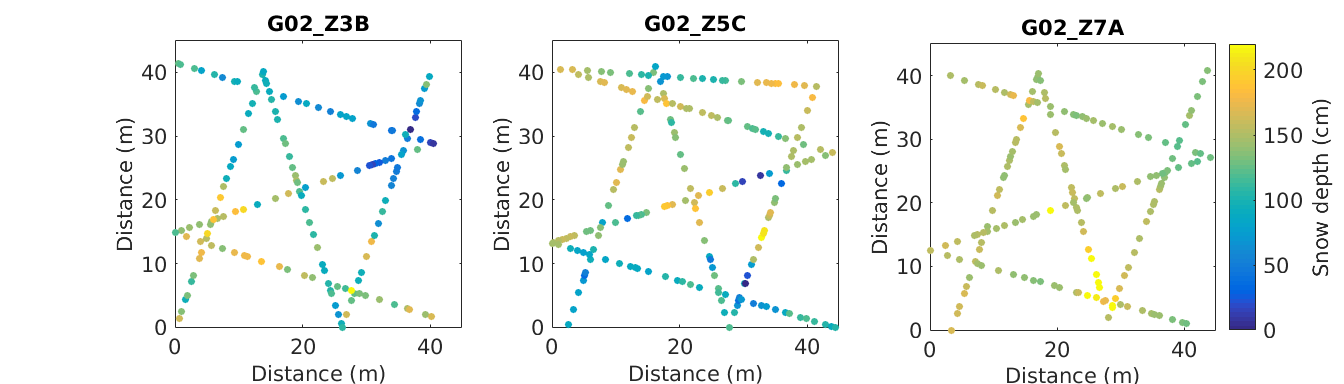
\includegraphics[width = 23 cm]{ZigzagDepth_G02.png}\\
	\caption{Plot of depth measured at zigzags on Glacier 2.}
	\label{fig:ZZ_G02}
\end{figure}
\end{landscape}

\begin{figure}[H] 
	\centering
	  \makebox[\textwidth][c]{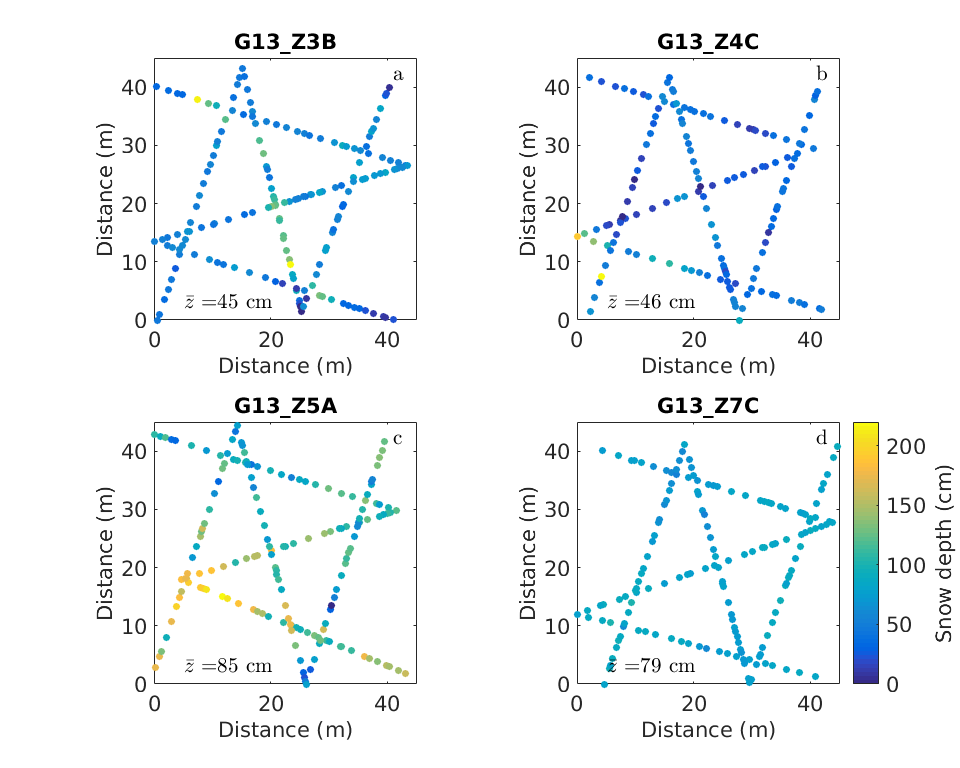
\includegraphics[width=1.1\textwidth]{ZigzagDepth_G13.png}}%
	\caption{Plot of depth measured at zigzags on Glacier 13.}
	\label{fig:ZZ_G13}
\end{figure}




\pagebreak
%%%%%%%%%%%%%%%%%%%%%%%%%%%%%%%%%%%%%%
\section{Snow water equivalent (SWE)}

Snow water equivalent (SWE) estimated for each sampling location can be seen in Figures  \ref{fig:SWEmap_S1} to \ref{fig:SWEmap_F4}. For maps of SWE calculated for each density option see the Appendix. Generally, SWE is highest on Glacier 4 and lowest on Glacier 13. Glacier 4 also shows considerable SWE variability within the basin, with both high and low values seen along a single transect. Note that the individual measurement locations overlap on the figure.

\begin{figure}[H]
	\centering
	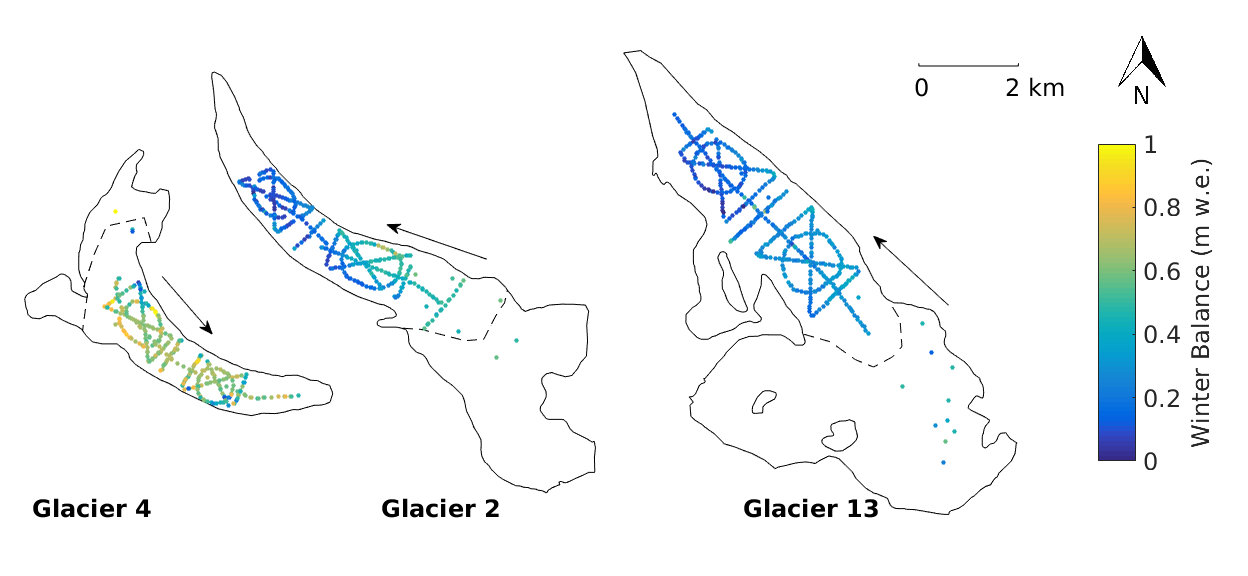
\includegraphics[width = \textwidth]{SWEmap_opt2.png}\\
	\caption{Estimated snow water equivalent (SWE) at measurement locations. Density was taken to be the mean value of all snowpit-derived densities (S1). Arrow shows ice flow direction.}
	\label{fig:SWEmap_S1}
\end{figure}

\begin{figure}[H]
	\centering
	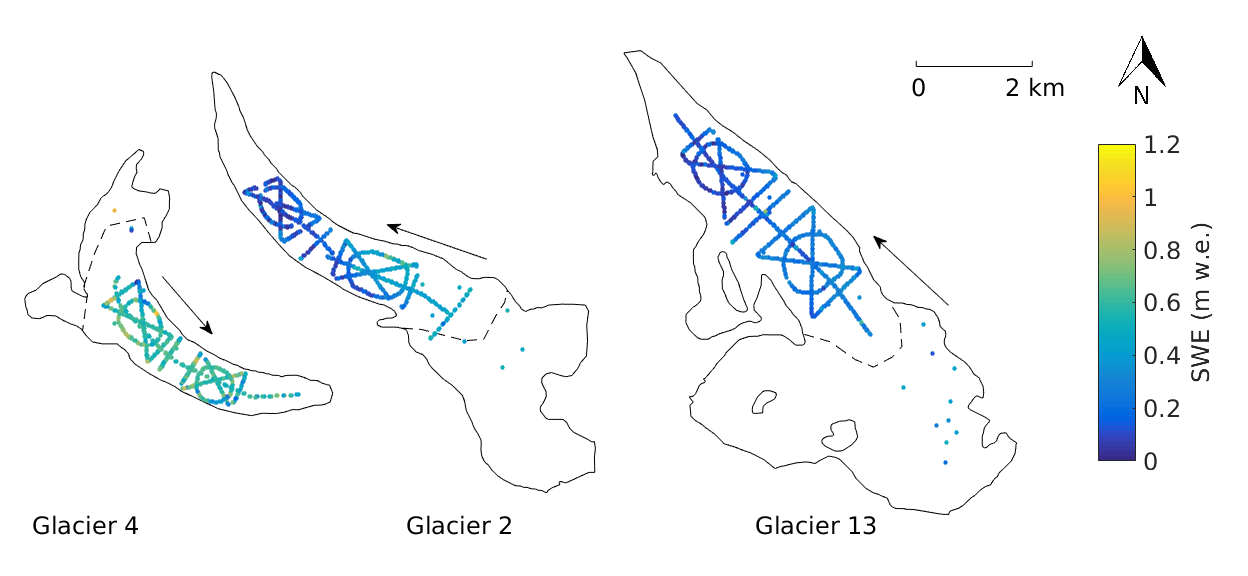
\includegraphics[width = \textwidth]{SWEmap_opt3.png}\\
	\caption{Estimated snow water equivalent (SWE) at measurement locations. Density was taken to be the mean value of all snowpit-derived densities (F1). Arrow shows ice flow direction.}
	\label{fig:SWEmap_F1}
\end{figure}

\begin{figure}[H]
	\centering
	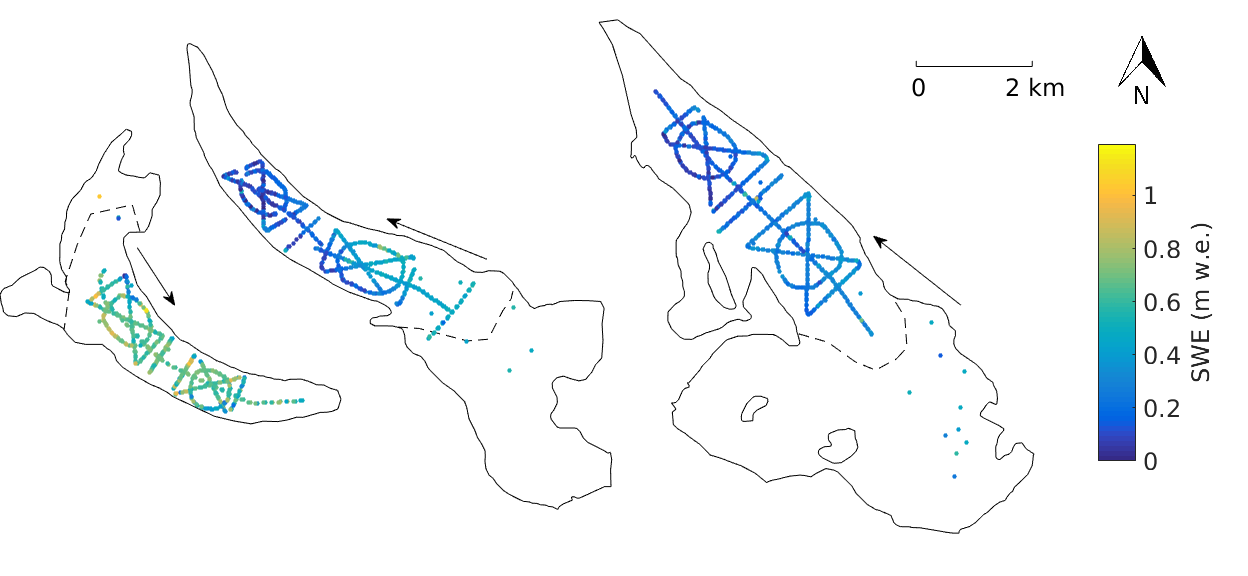
\includegraphics[width =\textwidth]{SWEmap_opt4.png}\\
	\caption{Estimated snow water equivalent (SWE) at measurement locations. Density was taken to be the mean value of snowpit-derived densities for each glacier (S2). Arrow shows ice flow direction.}
	\label{fig:SWEmap_S2}
\end{figure}

\begin{figure}[H]
	\centering
	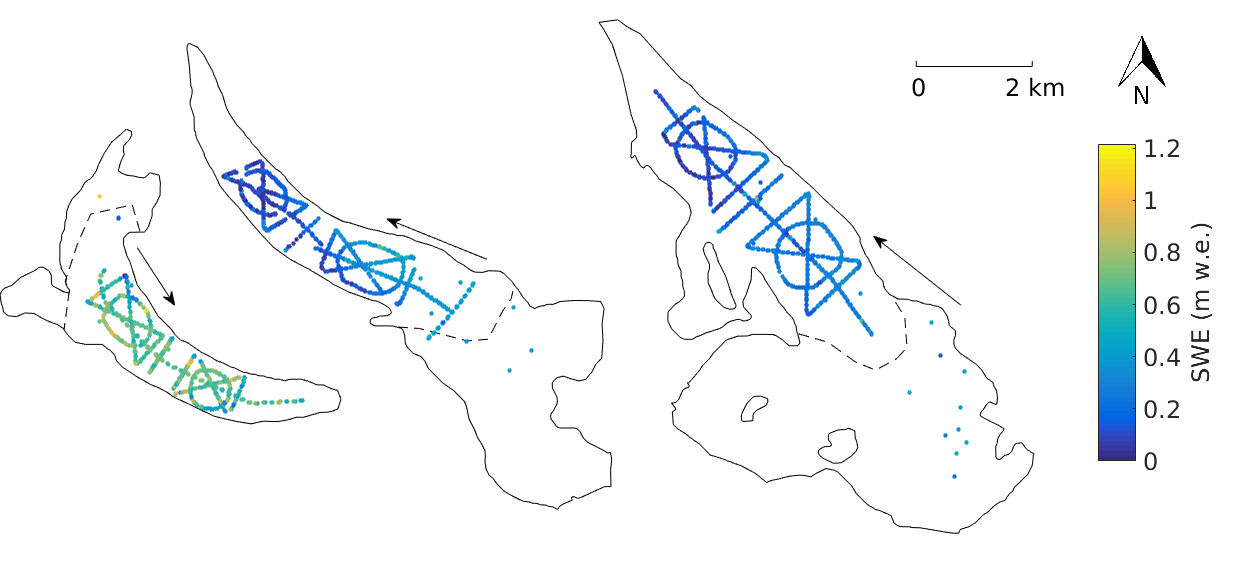
\includegraphics[width = \textwidth]{SWEmap_opt5.png}\\
	\caption{Estimated snow water equivalent (SWE) at measurement locations. Density was taken to be the mean value of Federal Sampler-derived densities for each glacier (F2). Arrow shows ice flow direction.}
	\label{fig:SWEmap_F2}
\end{figure}

\begin{figure}[H]
	\centering
	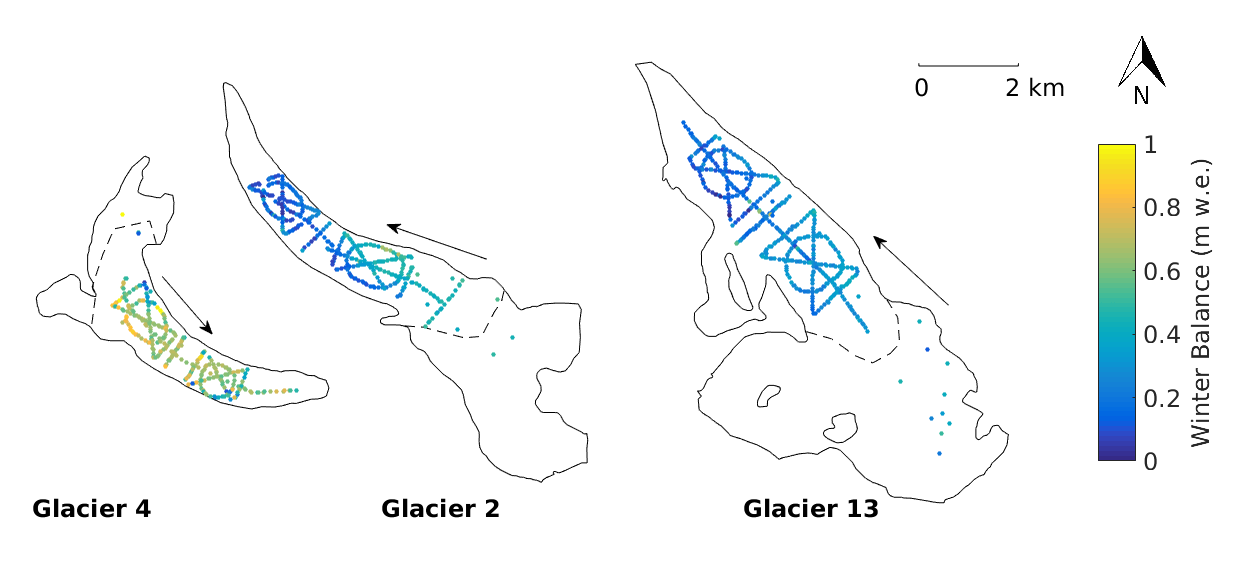
\includegraphics[width = \textwidth]{SWEmap_opt6.png}\\
	\caption{Estimated snow water equivalent (SWE) at measurement locations. Density was determined by using a linear fit between snowpit-derived density and elevation for each glacier (S3). Arrow shows ice flow direction.}
	\label{fig:SWEmap_S3}
\end{figure}

\begin{figure}[H]
	\centering
	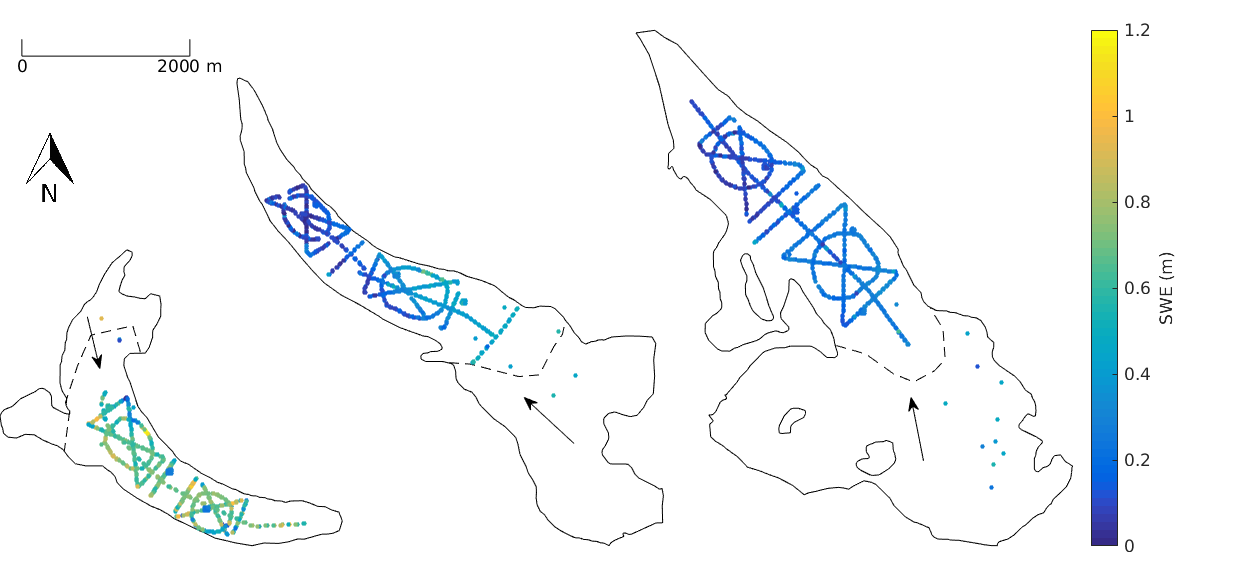
\includegraphics[width = \textwidth]{SWEmap_opt7.png}\\
	\caption{Estimated snow water equivalent (SWE) at measurement locations.Density was determined by using a linear fit between Federal Sampler-derived density and elevation for each glacier (F3). Arrow shows ice flow direction.}
	\label{fig:SWEmap_F3}
\end{figure}

\begin{figure}[H]
	\centering
	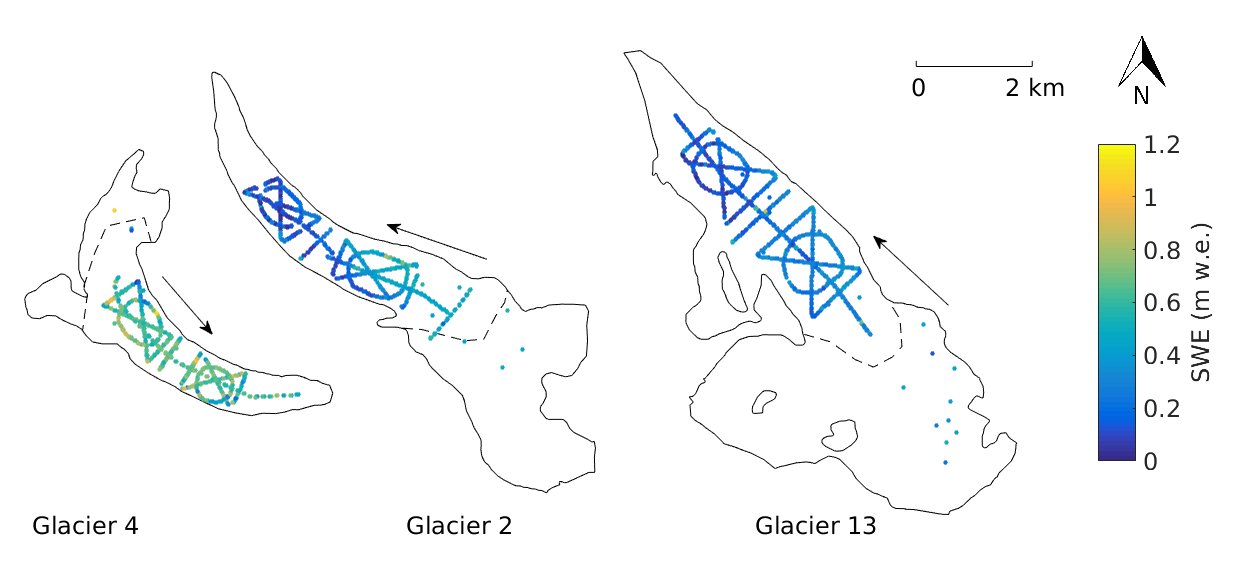
\includegraphics[width = \textwidth]{SWEmap_opt8.png}\\
	\caption{Estimated snow water equivalent (SWE) at measurement locations. Density was calculated using inverse distance weighting using all snowpit-derived densities (S4). Arrow shows ice flow direction.}
	\label{fig:SWEmap_S4}
\end{figure}

\begin{figure}[H]
	\centering
	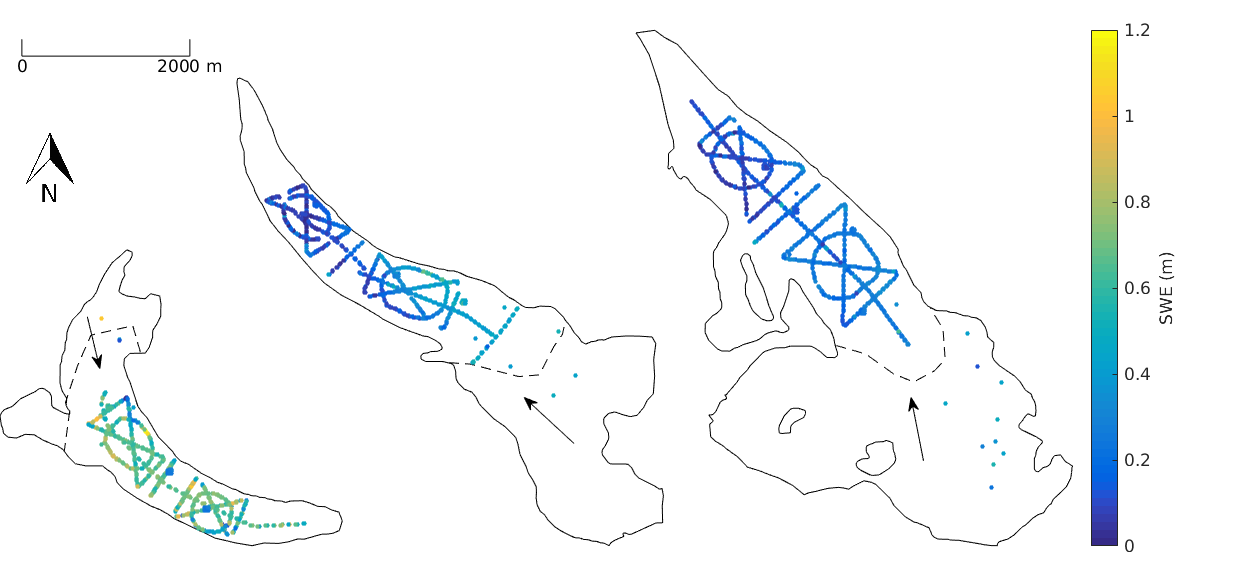
\includegraphics[width =\textwidth]{SWEmap_opt9.png}\\
	\caption{Estimated snow water equivalent (SWE) at measurement locations. Density was calculated using inverse distance weighting using all snowpit-derived densities (F4). Arrow shows ice flow direction.}
	\label{fig:SWEmap_F4}
\end{figure}


\end{document}